\newpage
\section{Systembeschreibung im Zustandsraum}
\subsection{Mehrgrößensystem MIMO}


\begin{center}
	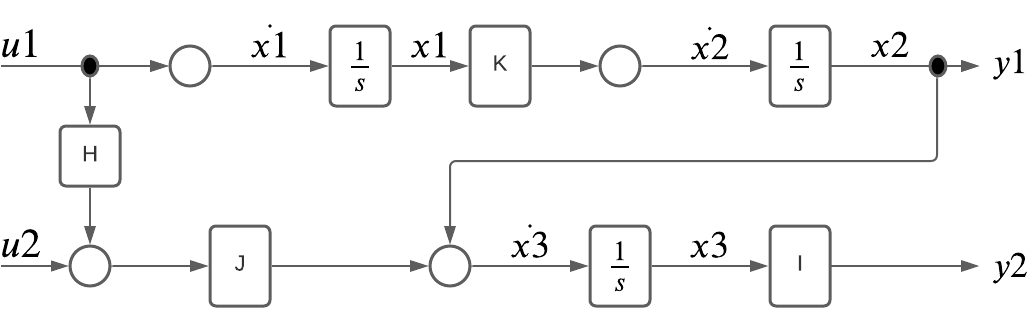
\includegraphics[width=1\columnwidth]{Figures/Signalflussplan.png}
	\captionof{figure}{Signalflussplan}
\end{center}

\subsubsection{Systemgleichungen}
\vspace{-1em}
\begin{align*}
	\dot{x}_{1} & = 0\cdot x_{1} +0\cdot x_{2} +0\cdot x_{3} +1\cdot u_{1}+0\cdot u_{2}        \\
	\dot{x}_{2} & = K\cdot x_{1} +0\cdot x_{2} +0\cdot x_{3} +0\cdot u_{1}+0\cdot u_{2}        \\
	\dot{x}_{3} & = 0\cdot x_{1} +0\cdot x_{2} +0\cdot x_{3} +H\cdot J\cdot u_{1}+J\cdot u_{2} \\
	\dot{y}_{1} & = 0\cdot x_{1} +1+x_{2} +0\cdot x_{3} +0\cdot u_{1}+0\cdot u_{2}             \\
	\dot{y}_{2} & = 0\cdot x_{1} +0\cdot x_{2} +l\cdot x_{3} +0\cdot u_{1}+0\cdot u_{2}        \\
	\vspace*{1em} \\
	\dot{\Vec{x}}(t) & = A\vec{x}(t) + B\vec{u}(t) \quad x(0) = x_{0} \\
	\vec{y}(t)       & = C\vec{x}(t) + D\vec{u}(t)
\end{align*}

\vspace{-1em}
\begin{mdframed}[style=exercise]
	\vspace{-1em}
	\subsubsection{Zustandsraumdarstellung}
	\begin{align*}
		A &= \begin{bmatrix}
			0 & 0 & 0 \\
			K & 0 & 0 \\
			0 & 0 & 0
		\end{bmatrix}
		\quad
		B = \begin{bmatrix}
			1         & 0 \\
			0         & 0 \\
			H\cdot{}J & J
		\end{bmatrix} 					\\
		C &= \begin{bmatrix}
			0 & 1 & 0 \\ 
			0 & 0 & l \\
		\end{bmatrix}
		\qquad
		D = \begin{bmatrix}
			0 & 0 \\
			0 & 0
		\end{bmatrix}
	\end{align*}
	
	Polstellen (Eigenwerte einer Matrix bestimmen):
    \[
        \operatorname{det}(A - sE)= \operatorname{det}
		\begin{bmatrix}
			a-s & b \\
			c & d-s \\
		\end{bmatrix} = (a-s)(d-s) - cb \overset{!}{=} 0
    \]
\end{mdframed}

\subsection{Programmtechnische Umsetzung}
\begin{align*}
	F_z(z) &= \frac{2z + 6}{3z + 4} = \frac{2x_{e,k} + 6x_{e,k-1}}{3x_{a,k} + 4x_{a,k-1}}\\
	3x_{a,k} + 4x_{a,k-1} &= 2x_{e,k} + 6x_{e,k-1} \\
	x_{a,k} &= \frac{2}{3}x_{e,k} + \frac{6}{3}x_{e,k-1} - \frac{4}{3}x_{a,k-1}
\end{align*}


\begin{lstlisting}[language=c]
while(1)
{
	waitinterrupt(T_A) 	//Abtastzeit warten
	x_a2 = x_a1			// ggf. nicht noetig
	x_a1 = x_a
	x_e2 = x_e1			// ggf. nicht noetig
	x_e1 = x_e
	input(x_e)
	x_a = k*x_e + j*x_e1 - o*x_a1
	output(x_a)
}
\end{lstlisting}